%
% This docuement is based on the Insight Journal Template.
% https://github.com/InsightSoftwareConsortium/InsightJournalTemplate/tree/ModularTemplate
% 4555fc04b105b11f06dc302b76bf09c27e50727d

\documentclass{InsightArticle}

\usepackage[dvips]{graphicx}
%  hyperref should be the last package to be loaded.
\usepackage[dvips,
bookmarks,
bookmarksopen,
backref,
colorlinks,linkcolor={blue},citecolor={blue},urlcolor={blue},
]{hyperref}

\title{The BinShrinkFilter: A multi-resolution filter with efficient averaging. }

\newcommand{\IJhandlerIDnumber}{0}

\release{0.00}

% At minimum, give your name and an email address.  You can include a
% snail-mail address if you like.
\author{Bradley C. Lowekamp$^{1}$ and David T. Chen$^{1}$}
\authoraddress{$^{1}$National Library Of Medicine}

\begin{document}

%
% Add hyperlink to the web location and license of the paper.
% The argument of this command is the handler identifier given
% by the Insight Journal to this paper.
% 
\IJhandlefooter{\IJhandlerIDnumber}


\ifpdf
\else
   %
   % Commands for including Graphics when using latex
   % 
   \DeclareGraphicsExtensions{.eps,.jpg,.gif,.tiff,.bmp,.png}
   \DeclareGraphicsRule{.jpg}{eps}{.jpg.bb}{`convert #1 eps:-}
   \DeclareGraphicsRule{.gif}{eps}{.gif.bb}{`convert #1 eps:-}
   \DeclareGraphicsRule{.tiff}{eps}{.tiff.bb}{`convert #1 eps:-}
   \DeclareGraphicsRule{.bmp}{eps}{.bmp.bb}{`convert #1 eps:-}
   \DeclareGraphicsRule{.png}{eps}{.png.bb}{`convert #1 eps:-}
\fi


\maketitle


\ifhtml
\chapter*{Front Matter\label{front}}
\fi

% The abstract should be a paragraph or two long, and describe the
% scope of the document.
\begin{abstract}
\noindent
This document describes a new algorithm not currently in itk\cite{ITKSoftwareGuide}. 
\end{abstract}

\IJhandlenote{\IJhandlerIDnumber}

\tableofcontents

Using filters from the Insight Toolkit, we develop an algorithm for detecting
and tracking thje movement of solar spots. As it is widely known, celestial
objects such as the sun are ethereal and perfect, and therefore can not harbor
artifacts such as spots. However, observations performed with our open source
telescope have revealed the presence of such spots. The spots seems to continuously change positions on the solar surface. 


Multi-resolution

why is this fitlter useful?

\section{Implementation}

Algorithm

Features

\subsection{Geometry}

\subsection{Optimization}
Optimization 


\section{Results}

Lets look as some image.

\subsection{Performance}

\section{Conclusion}

trade offs 



%%%%%%%%%%%%%%%%%%%%%%%%%%%%%%%%%%%%%%%%%%%%%%%%%%%%%%%%%%
%
%  Example on how to insert a figure
%
%%%%%%%%%%%%%%%%%%%%%%%%%%%%%%%%%%%%%%%%%%%%%%%%%%%%%%%%%%

\begin{figure}
  \centering
  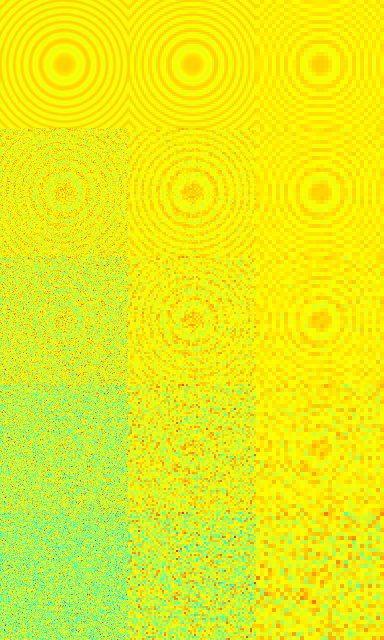
\includegraphics[width=0.4\linewidth]{images/binshrink_hot.png}
  \caption[Registration Framework Components]{The basic components of the
    registration framework are two input images, a transform, a metric, an
    interpolator and an optimizer.}
  \label{fig:BinShrinkComparison}
\end{figure}

\begin{figure}
  \centering
  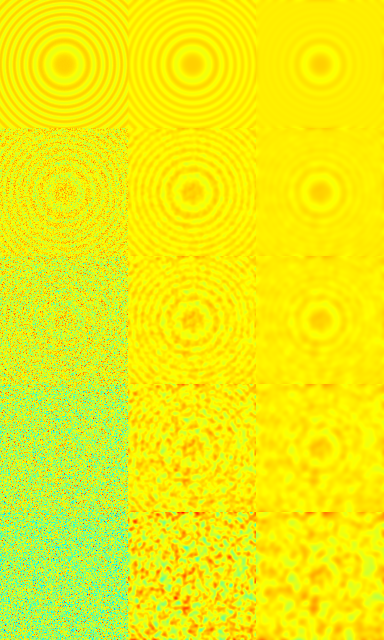
\includegraphics[width=0.4\linewidth]{images/gaussianshrink_hot.png}
  \caption[Registration Framework Components]{The basic components of the
    registration framework are two input images, a transform, a metric, an
    interpolator and an optimizer.}
  \label{fig:GaussianShrinkComparison}
\end{figure}


To support shape-guidance, the generic level set equation
(Eqn(~\ref{eqn:ShapeInfluenceTerm})) is extended to incorporate a shape guidance
term:

\begin{equation}
\label{eqn:ShapeInfluenceTerm}
\xi \left(\psi^{*}(\mathbf{x}) - \psi(\mathbf{x})\right)
\end{equation}




%%%%%%%%%%%%%%%%%%%%%%%%%%%%%%%%%%%%%%%%%
%
%  Insert the bibliography using BibTeX
%
%%%%%%%%%%%%%%%%%%%%%%%%%%%%%%%%%%%%%%%%%

\bibliographystyle{plain}
\bibliography{BinShrink}


\end{document}

